\chapter{Moving to the Web}
We decided to build Giflang's interpreter and the IDE for web and we tried to move as much code to the client side as possible, resulting in a server that
simply serves static files. This chapter sheds light on why we decided to do so.

We believe that the usage of web browsers compared to other desktop apps is very high.\footnote{We did not
find any statistics backing up this statement. /TODO: Try harder/} Google is even building an operating system called ChromeOS based around their
market-dominating browser Chrome. With modern Web APIs, apps that were previously thought of as typical desktop apps are now moving to the browser. Below
are a few examples of such apps:
\begin{enumerate}
\item Photopea \cite{Photopea} -- A Photoshop web alternative
\item Google Hangouts \cite{Hangouts} -- A pioneer WebRTC\footnote{WebRTC (Web Real-Time Communication) provides web browser 
applications with real-time communication (RTC) via simple APIs.} app providing realtime video communication
\item TODO: Add an in-browser FPS here
\end{enumerate}

\section{Native vs Web IDE}
Most well known IDEs (e.g., Visual Studio, Eclipse or Xcode) are desktop applications. Web IDEs such as REPL.it or Ideone, on the other hand,
are not very widespread. We think that this is because users usually want to edit local files while browsers have limited support for reading
and saving local files programmatically. There is no Web API to overwrite a file at a given location on a user's disk for example.
Browsers prohibit this to protect the user's security.

Giflang is not suited for use in any serious project development and it is also not intended for such use. It is meant for creating
challenging and fun environment for solving programming problems. Standard I/O can be used for accepting problem inputs and writing results.

Therefore, Giflang does not have to support file I/O, multi-source programs and other otherwise-standard functionality. Of course later
on a graphical output, file I/O or other features can be added, but within the scope of this thesis we only plan on supporting
basic functionality.

Considering the above paragraphs we concluded that web IDE is more suitable for our type of application since it offers benefits as
ease of access and installation-free setup. In our opinion this outweighs the advantages of desktop IDEs such as easy local disk
file access and higher performance.

\section{Client side vs server side interpreter}

The Giflang code can be either interpreted on the server side or client side. By server side we mean any code that runs on the server. This means that
the interpret could be written in almost any language using any technologies, because it is up to us to choose what we run on the server. On the other hand,
client side code is executed in the browser which can only run JavaScript or WebAssembly.

\subsection{Server side execution}
Executing code on the server side means that in order to interact with it (e.g., provide interactive input or see gradual output) browser and
server need to communicate during the execution. There are $2$ basic approaches to this communication:
\begin{enumerate}
\item HTTP polling -- client (browser) initiates the communication to the server and waits for a response
\item WebSockets -- client and server open a two-way channel (WebSocket) through which the server can send messages to the client without
the client sending a request 
\end{enumerate}

\begin{figure}[!hbt]
	\includegraphics[width=\textwidth]{../img/websockets}
	\caption{Difference between using HTTP polling and WebSockets}
	\label{fig:chap1:websockets}
\end{figure}

We will introduce two Web IDEs that use server side execution -- REPL.it and Ideone. They both support numerous languages such
as Python, C, C++ and Java.

Ideone uses HTTP polling to get updates about the execution. Firstly, it sends a request to the backend containing source code and input.
After that it polls the server for an update every second. The server can respond with new output, error report, finish status, etc. Users of Ideone need to
specify all the output at once before the start. While it would be possible to implement interactive IO with the polling Ideone chose not to do so.
We did not find out why.

Having to poll the server for updates is awkward. If the granularity of polling is high requests are send frequently, but
in between consecutive requests the state might not have changed. That results in wasting resources. On the other hand, if the granularity is low less
requests are send, but that might result in higher latency between a state change happening on the server and the client picking it up.

WebSockets address this issue. They allow opening a two-way interactive communication session between the user's browser and a server.
With this API, browser can send messages to a server and receive event-driven responses without having to poll the server for a reply\footnote{source: mdn todo}.
You can see this in Figure \ref{fig:chap1:websockets} where WebSocket communication is marked with red arrows.
Before WebSockets were introduced around the year 2012 there was not a way to initiate a communication from server to browser as HTTP is a request-response
protocol. This means that server can only respond to browser's requests.

REPL.it is more modern compared to Ideone and uses WebSockets. It also provides interactive IO and debugging.

\subsection{Client side execution}
By default, the browser uses a single thread -- also called the main thread -- to run all the JavaScript in user's page, as well as to perform layout
changes, reflows, and garbage collection. As a result of this, long-running JavaScript functions can block the thread, leading to an unresponsive page and
a bad user experience.\footnote{source: mdn}

\subsubsection{WebWorkers}
Running the interpreter in the main thread would take processing time from UI updates which could lead to a bad responsiveness of the site. To
address this issue, browsers adopted support for WebWorkers. WebWorkers allow us to run scripts in the background threads, leaving main thread
to handle UI-related tasks.

Sharing data between threads is typically achieved by accessing the same piece of memory. However, communication between WebWorkers and the main
thread is achieved via messages:
\begin{code}
// Main script
var myWorker = new Worker('worker.js');
myWorker.postMessage('Hello Worker');

// worker.js
onmessage = function(msg) {
  console.log('Got a message from main: ' + msg);
}
\end{code}

An interpreter running in a separate WebWorker does not take processing time from the UI tasks in the main thread. We could not find an existing
project that would interpret or compile code in a WebWorker.

\subsubsection{WebAssembly}
JavaScript in the browser is executed by a JavaScript engine. Different browsers might have different engines. As Figure \ref{fig:chap2:v8_bench} shows,
JavaScript engines like V8 or SpiderMonkey keep improving in terms of speed. Nonetheless, a program written in a language
with highly optimized compiler like C++ or Rust that compiles to machine code will most probably outperform any JavaScript engine.

\begin{figure}[!hbt]
	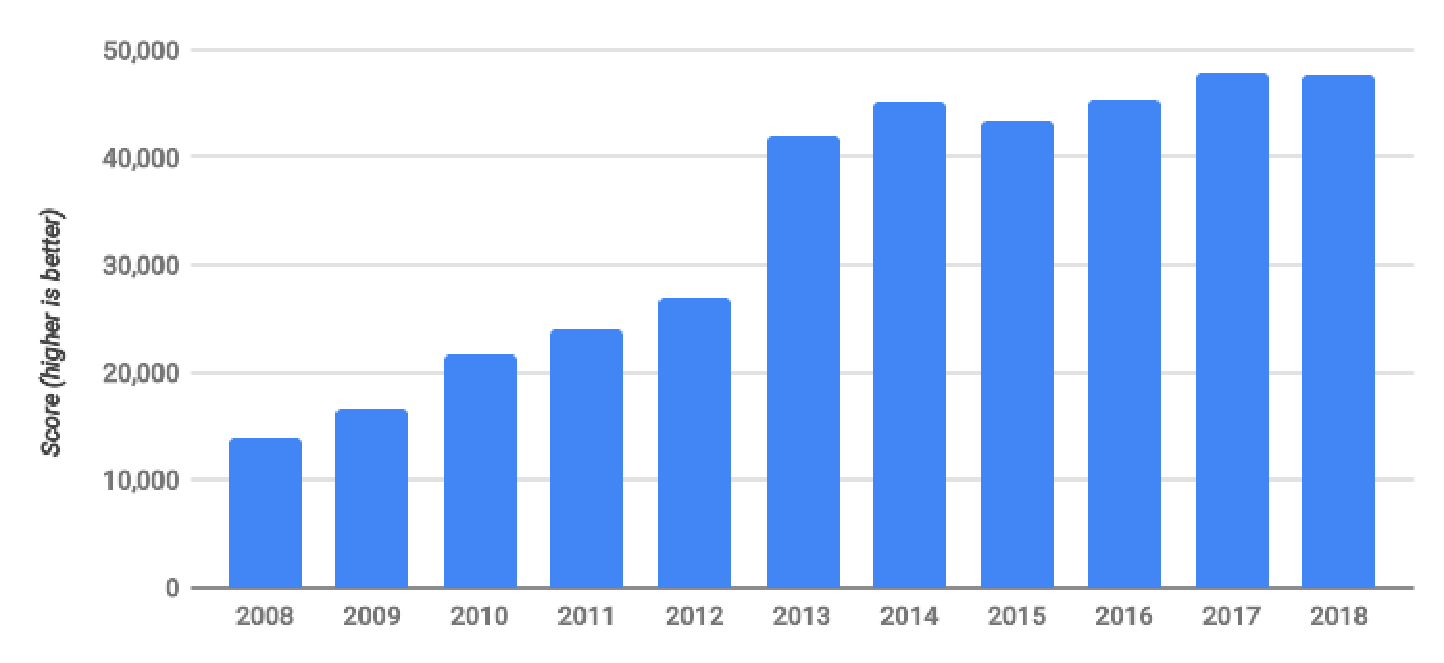
\includegraphics[width=\textwidth]{../img/v8-bench}
	\caption{A chart showing V8 improving over the years. Source: \href{https://v8.dev/blog/10-years}{v8.dev}}
	\label{fig:chap2:v8_bench}
\end{figure}

In order to close the gap between computational-heavy programs executing well natively while poorly in browser, WebAssembly
language was introduced in 2015. WebAssembly is a low level language that is now supported by all major browsers. Since it is
close to machine code, it is meant to be a compilation target language of other higher level languages.

Currently, many languages such as C/C++, Rust or TypeScript, can be compiled to WebAssembly. These compilers typically also emit
a `glue code' that contains handles that allow calling functions defined in the WebAssembly code from JavaScript.

Integrating functions defined in WebAssembly into a JavaScript script requires non-trivial effort since only primitive types can be passed
as function arguments and return values.

There are many ports of existing interpreters and compilers to WebAssembly, because there are tools like Emscripten\footnote{Add reference}
that can compile C/C++ code to WebAssembly. For example we really like Iodide\footnote{Todo reference} project that brings scientific Python
to the client side of the browser.

\subsection{Conclusion}
The advantage of server side interpreter is speed as the interpreter can use almost any technology. Web IDEs typically choose
server side execution for different reason, though. It is simpler than implementing interpreters for given languages in JavaScript or
porting the existing interpreters to WebAssembly. Since in our project we do not care so much about execution speed and
we do not have an existing interpreter or compiler, we can do better than server side execution.

The client side execution requires no special support from the server and it also works offline, i.e., after user looses connection. Running an interpreter
compiled to WebAssembly in a WebWorker would be the best approach as it would provide performance and also offloading from the main thread.
However, when we started working on the thesis we did not have any prior experience with writing an interpreter and adding another layer into the stack in the
form of WebAssembly seemed very complex. It would allow us to use language like C++ or Rust for the development, though. To keep things simpler we
decided to write the interpreter in JavaScript and run it in a WebWorker.

\section{Picking the right Javascript flavour}
Why typescript is awesome.


\section{Frontend framework vs vanilla Javascript}

\subsection{Frontend Frameworks Struggle}
Why react and how does it work

\section{Storing programs}

\subsection{Firebase vs typical storage model}

\subsection{Encoding program id in the URL}